\section{Deep learning for DIA}

Goal: Overview of DIA tasks addressed by deep learning, network architectures
to do so.

\subsection{Autoencoders}

\begin{itemize}
		\item Symmetrical network, trained to recover input from compressed intermediate code
		\item A form of universal feature extractor. Reduces information in a
				way that the `compressed' form is as representative as possible
		\item Outperformed by more specific systems
\end{itemize}

\subsection{Residual neural network}

\begin{itemize}
		\item Convolutional networks with shortcuts to jump over some layers
		\item Shortcuts of length 2 empirically improve performance: Faster
				training, better generalization.
		\item Pretrained networks exist for image analysis
\end{itemize}

\subsection{U-Net}

\begin{itemize}
		\item Several modules, combined by a contracting path (convolutional
				layers, ReLU activation, pooling layers) and expansive path
				(deconvolution).
		\item U-shape. Left half is contracting path, second half is expanding
				path.
\end{itemize}

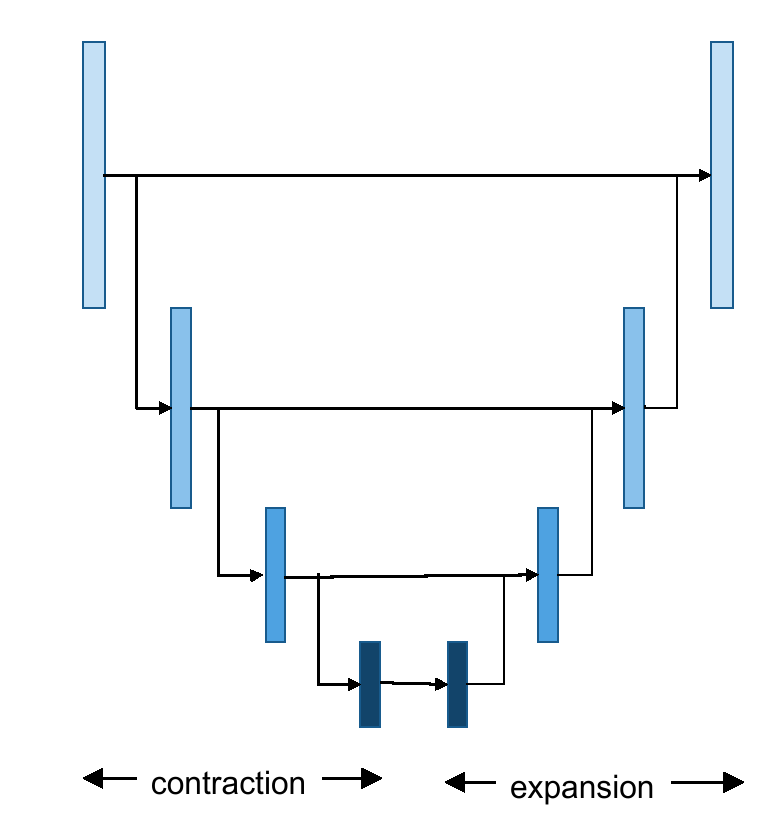
\includegraphics[width=0.5\textwidth]{11_unet}

\subsection{Siamese networks}

\begin{itemize}
		\item Composed of two identical subnetworks with shared weights
		\item Extract feature vector of two similar inputs
		\item Also learn a dissimilarity measure between their two outputs
		\item Well adapted when low amount of data (e.g. signature or face
				recognition)
\end{itemize}

\subsection{Triplet loss function}

\begin{itemize}
		\item Alternative for CNNs, can map input to vector space
		\item Then dissimilarity is measure between vectors in embedded space
		\item Models trained by comparing anchro point with positive and
				engative sample, and minimizing triplet loss function $L(a, p,
				n) = \max(d(a, p) - d(a, n) + margin, 0)$
		\item Anchor $a$ might e.g. be reference image of signature, positive a
				second example, negative a forgery
\end{itemize}

\subsection{GAN}

\begin{itemize}
		\item Used to generate synthetic data
		\item Competing networks, discriminator is trained to distinguish real
				and fake samples, generator is trained to fool the
				discriminator.
		\item Training is computing-intensive and can be tricky
\end{itemize}

\subsection{Semantic layout analysis}

Goal: Detect and classify regions, e.g. background, text blocks, lines,
decorations, ... Different networks:

\begin{description}
		\item[CNN] Sliding window, 3-layer encoder, 1 fully connected hidden
				layer, 1 softmax output layer.
		\item[Asymmetric u-net] 6 convolution layers, 2 deconvolution layers,
				trained with MSE
\end{description}

\subsection{Semantic segmentation}

Goal: Split image into regions. E.g. cat picture into `cat', `sky', `trees',
`grass'.

Approaches:
\begin{description}
		\item[U-Net], evaluation with mean intersection over union: $mIU =
				|C|^{-1} \cdot \sum IU_c$, where $IU_c = \frac{TP_c}{TP_c +
				FP_c + FN_c}$
\end{description}

\subsection{Text line segmentation}

Starting with pixel-wise segmentation, achieve text segmentation of historical
documents.

\subsubsection{Seam carving}

\begin{itemize}
		\item DP, cheapest path through image
		\item Only walk forward, no looking ahead, no backtracking
\end{itemize}

\subsubsection{ML approach}

\begin{enumerate}
		\item Pixel to energy map from segmentation output, text gets high energy, background low energy
		\item Start seam carving every $x$ pixel. Assume seams find lines even
				if they are spaced slightly unevenly
				\begin{itemize}
						\item `Punish' seams for leaving straight path
						\item Release seams from both sides
				\end{itemize}
		\item Collect lines into clusters, generate bins
		\item Get connected components of each bin, connect them with minimum
				spanning three from CC centers, results in (hopefully) one CC
				per line
\end{enumerate}

Evaluation as IoU, average pixel recall and precision, average line recall and
precision.
